% !TEX root = ../main.tex

% \begin{table*}[b]%
%     \begin{DndTable}[width=\linewidth]{X}
%         \centering
%         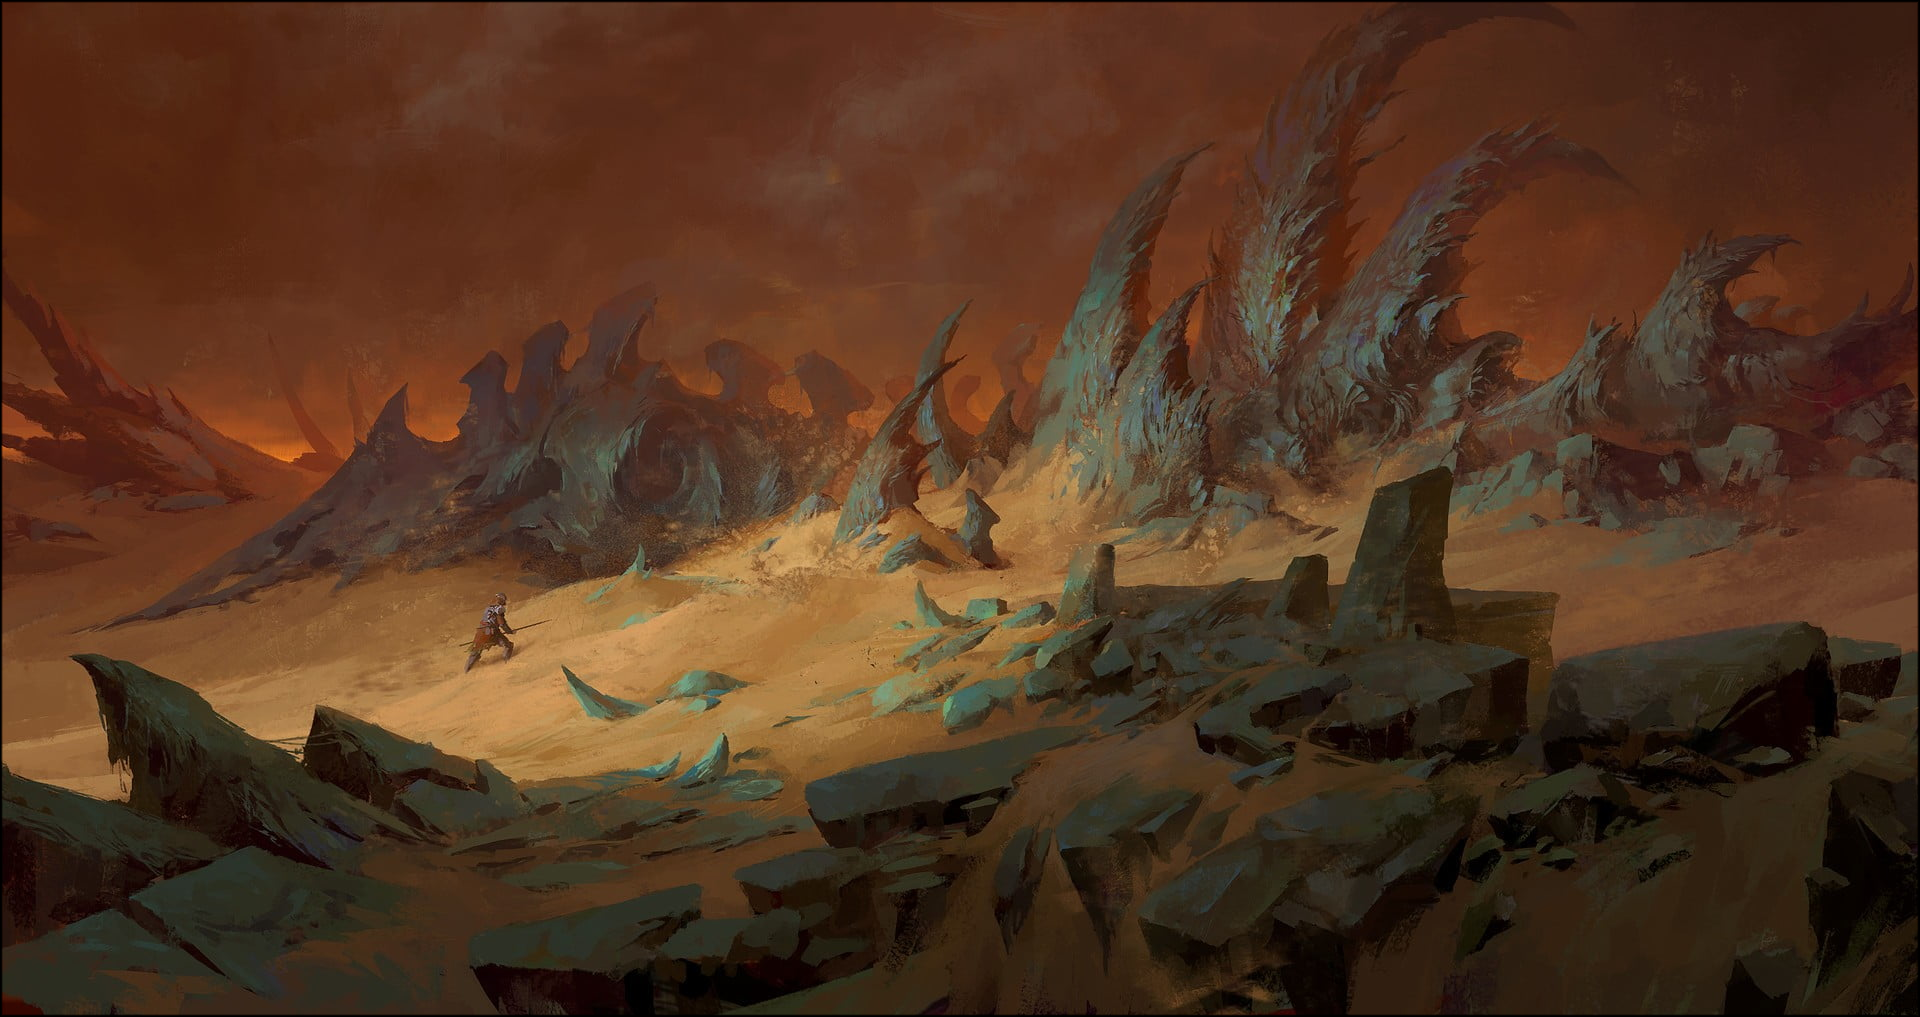
\includegraphics[width=0.95\textwidth]{01yuadrem/img/12dead_sea.png} \
%         \centering \large{\textbf{The Bone Cliffs of the Dead Sea}}
%     \end{DndTable}
% \end{table*}

\subsection*{The Three Deserts} \label{ssec::threedeserts}
Effectively splitting Yuadrem in half are the three deserts: Zoedrem, Zashlath, and the Dead Sea.

Zoedrem is a large expanse of yellow sands the embraces the waves of both the Whaler's Sea and the Teal Ocean.
The desert runs undisturbed from the Sulfur Lake down to the Defiled River.
It is commonly regarded as the most forgiving of the three deserts.

More fearsome than the sands are its inhabitants, the five dratl ird houses of Zoedrem.
Descendants of the fallen empire of Hulnar, they hide their settlements along the stone cliffs.
They are constantly in search of prey, robbing and murdering any traveler foolish enough to travel in their territories.

At the easternmost point of Zoedrem is the Sylvan Canyon, the only area in the desert able to host life.
The gorge is the home of the independent nation of Viphoger.
Apart from its inhabitants, the canyon's soil has rich natural deposits of oil, salt, and gemstones.
These resources grant Viphoger a strong economy despite its young age.

Southeast of Zoedrem and across the Ichor Mountains lie the Dead Sea, an artificial desert created by the tall kin's folly.
The desert's sands are of a sickly gray color, and any creature that inhabit the land for too long suffer particular mutations.
Its inhabitants, the treb gats and the cursed umans are perhaps the best examples of this.

The sands become blacker the more you approach the spire, the largest mountain in Yuadrem.
The et city of Jan'krug stands atop it, where the ritual that caused the Schism took place.
A long chasm divides the eastern region of the Dead Sea, remnants of the passage of the breathing island, Cabb Goem-Rlamesh.
Surrounded by hill, mountain, and river, the desert naturally prohibits passage to it, almost as if it's protecting a twisted secret.

Apart from the kins that call this desert home, the Dead Sea is infested with other monstrosities.
These are categorized into two: The Nyxborn and the children of Cabb.
The former are giant insect-like creatures that can be as large as an elephant and as precise as a mosquito.
The latter are tormented amalgamates that dislodged from Cabb Goem-Rlamesh, ever haunted by insatiable hunger and unending pain.

% Along with the tortles, grungs, and umans, the Schism brought forth terrible creatures known as the Nyxborn.
% These insect-like monstrosities can be as huge as the Mirmekolon, a colossal ant-lion hybrid, or as precise as the Khanokoladtes, a palm-sized moth that pierces skulls with its sharp dart-like mouth.

South, through the Hammerfall canyon, is the Zashlath desert, the driest of the three.
Featureless and white, only the hardy sunstruck oths have been able to call the desert home, and even they are wise enough to only establish by the neighboring mountains.

Zashlath practically receives no precipitation, and its white-colored sands reflect the scorching sunlight to deadly effect.
Truth is the desert remains largely unexplored to this date, and only rumors exist about the horrors that might hide among its sands.
Famous among these is the Haimorrois, a red horned snake whose bite forces the blood out of one's body.
